%&../preamble

\def\npart {IB}
\def\nterm {Michaelmas}
\def\nyear {2022}
\def\nlecturer {Dr P. Russell}
\def\ncourse {Analysis and Topology}

\def\encodingdefault{TU}\normalfont
\ifnum 0\ifxetex 1\fi\ifluatex 1\fi=0 % if pdftex
  \usepackage[T1]{fontenc}
  \usepackage[utf8]{inputenc}
  \usepackage{textcomp} % provide euro and other symbols
\else % if luatex or xetex
  % \usepackage{unicode-math}
  % \defaultfontfeatures{Scale=MatchLowercase}
  % \defaultfontfeatures[\rmfamily]{Ligatures=TeX,Scale=1}
  % \DeclareMathAlphabet{\mathcal}{OMS}{cmsy}{m}{n}
  % \let\mathbb\relax % remove the definition by unicode-math
  % \DeclareMathAlphabet{\mathbb}{U}{msb}{m}{n}
\fi

\usetikzlibrary{external}
\tikzset{external/system call={xelatex -fmt=../preamble.fmt \tikzexternalcheckshellescape -halt-on-error -interaction=batchmode -jobname "\image" "\texsource"}} % path is relative to file that includes preamble
\tikzexternalize

\providetoggle{DontSetTitleAuthorDate}

\nottoggle{DontSetTitleAuthorDate}{
  \hypersetup{
    pdftitle={Part \npart\ - \ncourse},
    pdfsubject={Cambridge Maths Notes: Part \npart\ - \ncourse},
    pdfkeywords={Cambridge Mathematics Maths Math \npart\ \nterm\ \nyear\ \ncourse}
  }

  \author{Based on lectures by \nlecturer}
  \date{\nterm\ \nyear}
  \title{Part \npart\ --- \ncourse}
}{}

\tikzsetexternalprefix{figtemp/}
\newcommand{\norm}[1]{\left \lVert #1 \right \rVert}
\usepackage{bbm}
% \includeonly{00-intro.tex}

% \setcounter{section}{-1}

\begin{document}
    \maketitle
    \tableofcontents

    \part{Generalizing continuity and convergence}
    \section{Three Examples of Convergence}
    \subsection{Convergence in $\mathbb{R}$}
    Let $(x_n)$ be a sequence in $\mathbb{R}$ and $x \in \mathbb{R}$.
    We say $(x_n)$ \textit{converges} to $x$ and write $x_n \to x$ if
    \begin{align*}
        \forall \; \epsilon > 0 \quad \exists \; N \quad \forall \; n \geq N \quad |x_n - x| < \epsilon.
    \end{align*} 
    Useful fact: $\forall \; a, b \in \mathbb{R} \ |a+b| \leq |a| + |b|$ (Triangle Inequality).

    Bolzano-Weierstrass Theorem (BWT)
    A bounded sequence in $\mathbb{R}$ must have a convergent subsequence (Proof by interval bisection).

    Recall: A sequence $(x_n)$ in $\mathbb{R}$ is Cauchy if 
    \begin{align*}
        \forall \; \epsilon > 0 \quad \exists \; N \quad \forall \; m, n \geq N \quad |x_m - x_n| < \epsilon.
    \end{align*} 

    Easy exercise Convergent $\implies$ Cauchy

    General Principle of Convergence (GPC)
    Any Cauchy sequence in $\mathbb{R}$ converges.

    \begin{proof}[Outline]
        If $(x_n)$ Cauchy then $(x_n)$ bounded so by BWT has a convergent subsequence, say $x_{n_j} \to x$.
        But as $(x_n)$ Cauchy, $x_n \to x$.
    \end{proof} 

    \subsection{Convergence in $\mathbb{R}^2$}
    \begin{remark}
        This all works in $\mathbb{R}^n$
    \end{remark} 

    Let $(z_n)$ be a sequence in $\mathbb{R}^2$ and $z \in \mathbb{R}^2$.
    What should $z_n \to z$ mean?

    In $\mathbb{R}$: ``As $n$ gets large, $z_n$ gets arbitrarily close to $z$.''

    What does `close' mean in $\mathbb{R}^2$?

    In $\mathbb{R}$: $a, b$ close if $|a - b|$ small.
    In $\mathbb{R}^2$: Replace $|\cdot|$ by $\left \lVert \cdot \right \rVert $

    Recall: If $z = (x, y)$ then $\left \lVert z \right \rVert = \sqrt{x^2 + y^2}$.

    Triangle Inequality If $a, b \in \mathbb{R}^2$ then $\left \lVert a + b \right \rVert \leq \left \lVert a \right \rVert + \left \lVert b \right \rVert$.

    \begin{definition}
        Let $(z_n)$ be a sequence in $\mathbb{R}^2$ and $z \in \mathbb{R}^2$.
        We say $(z_n)$ \vocab{converges} to $z$ and .. $z_n \to z$ if $\forall \; \epsilon > 0 \ \exists \; N \ \forall \; n \geq N \ \left \lVert z_n - z \right \rVert < \epsilon$. 

        Equivalently, $z_n \to z$ iff $\left \lVert z_n - z \right \rVert \to 0$ (convergence in $\mathbb{R}$).
    \end{definition} 

    \begin{example}
        Let $(z_n), (w_n)$ be sequences in $\mathbb{R}^2$ with $z_n \to z, w_n \to w$. 
        Then $z_n + w_n \to z + w$.
    \end{example} 

    \begin{proof}
        \begin{align*}
            \left \lVert (z_n + w_n) - (z + w) \right \rVert &\leq \left \lVert z_n - z \right \rVert + \left \lVert w_n - w \right \rVert \\
            &\to 0 + 0 = 0 \ \text{(by results from IA)}.
        \end{align*} 
    \end{proof} 

    In fact, given convergence in $\mathbb{R}$, convergence in $\mathbb{R}^2$ is easy:
    \begin{proposition} \label{prop:one}
        Let $(z_n)$ be a sequence in $\mathbb{R}^2$ and let $z \in \mathbb{R}^2$.
        Write $z_n = (x_n, y_n)$ and $z = (x, y)$.
        Then $z_n \to z$ iff $x_n \to x$ and $y_n \to y$.
    \end{proposition} 

    \begin{proof}
        ($\implies$): $|x_n - x|, |y_n - y| \leq \norm{z_n - z}$.
        So if $\norm{z_n - z} \to 0$ then $|x_n - x| \to 0$ and $|y_n - y| \to 0$.

        ($\Longleftarrow$): If $|x_n - x| \to 0$ and $|y_n - y| \to 0$ then $\norm{z_n - z} = \sqrt{(x_n - x)^2 + (y_n - y)^2} \to 0$ by results in $\mathbb{R}$.
    \end{proof} 

    \begin{definition}[Bounded Sequence]
        A sequence $(z_n)$ in $\mathbb{R}^2$ is \vocab{bounded} if $\exists \; M \in \mathbb{R}$ s.t. $\forall \; n \ \norm{z_n} \leq M$.
    \end{definition} 

    \begin{theorem}[BWT in $\mathbb{R}^2$]
        A bounded sequence in $\mathbb{R}^2$ must have a convergent subsequence.
    \end{theorem} 

    \begin{theorem}[GPC for $\mathbb{R}^2$]
        Any Cauchy sequence in $\mathbb{R}^2$ converges.
    \end{theorem} 

    \begin{proof}
        Let $(z_n)$ be a Cauchy sequence in $\mathbb{R}^2$.
        Write $z_n = (x_n, y_n)$.
        For all $m, n, |x_m - x_n| \leq \norm{z_m - z_n}$ so $(x_n)$ is a Cauchy sequence in $\mathbb{R}$, so converges by GPC.
        Similarly, $(y_n)$ converges in $\mathbb{R}$.
        So by \ref{prop:one}, $(z_n)$ converges.
    \end{proof} 

    \underline{Thought for the day} What about continuity?
    Let $f: \mathbb{R}^2 \to \mathbb{R}$.
    What does it mean for $f$ to be continuous?
    (Simple modification of defn for $\mathbb{R} \to \mathbb{R}$).

    What can we do with it?

    Big theorem in IA: If $f: \mathbb{R} \to \mathbb{R}$ is a continuous function on a closed bounded interval then $f$ is bounded and attains its bounds.

    Is there a similar theorem for $\mathbb{R}^2 \to \mathbb{R}$.
    What do we replace `closed bounded interval' by?
    We proved the theorem using BWT.
    Why did it work?
    Why did we need a closed bounded interval to make it work?
    What can we do in $\mathbb{R}^2$?

    \subsection{Convergence of Functions}
    Let $X \subset \mathbb{R}$\footnote{Mostly can think of $X = \mathbb{R}$ or some interval}, let $f_n : X \to \mathbb{R}$ ($n \geq 1$) and let $f: X \to \mathbb{R}$.
    What does it mean for $f_n$ to converge to $f$.

    Obvious idea:
    \begin{definition}[Pointwise convergence]
        Say $(f_n)$ \vocab{converges pointwise} to $f$ and write $f_n \to f$ pointwise if $\forall \; x \in X \ f_n(x) \to f(x)$ as $n \to \infty$.
    \end{definition} 

    Pros
    \begin{itemize}
        \item Simple
        \item Easy to check
        \item Defined in terms of convergence in $\mathbb{R}$
    \end{itemize} 
    Cons
    \begin{itemize}
        \item Doesn't preserve `nice' properties.
        \item `Doesn't feel right'.
    \end{itemize} 

    In all three examples, have $X = [0, 1], f_n \to f$ pointwise.

    \begin{example}[Every $f_n$ continuous but $f$ not] ~\vspace*{-1.5\baselineskip}
        \begin{align*}
            f_n(x) &= \begin{cases}
                nx & x \leq \frac{1}{n} \\
                1 & x \geq \frac{1}{n}
            \end{cases} \\
            f(x) &= \begin{cases}
                0 & x= 0 \\
                1 & x> 0
            \end{cases} 
        \end{align*} 
        {\par
            \centering 
            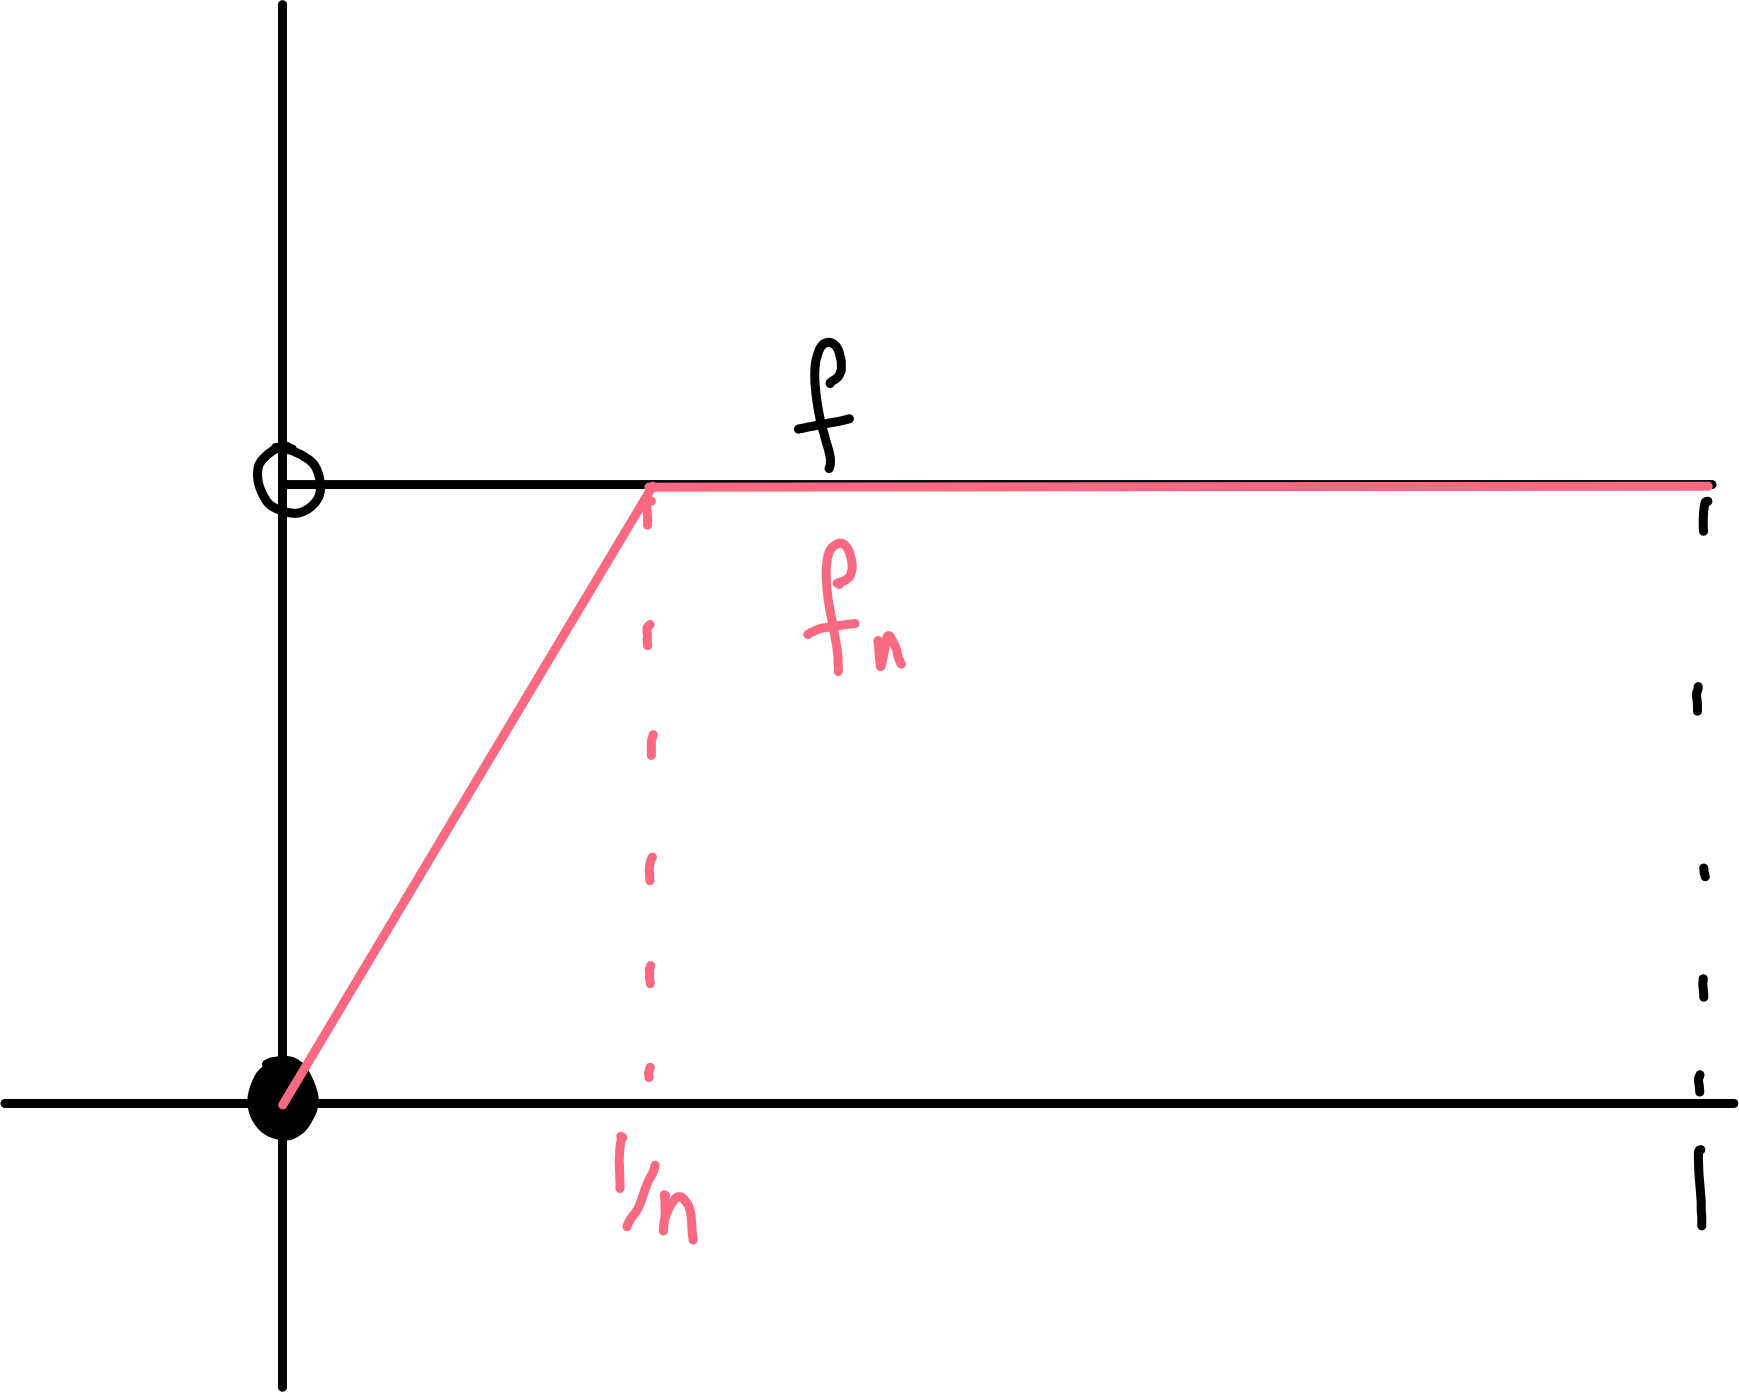
\includegraphics[height=5cm]{01-pointwise1} 
        \par}
        Clearly $f_n$ continuous for all $n$ but $f$ not.
        If $x = 0,\ \forall \; n \ f_n(0) = 0 = f(0)$.
        If $x > 0$, for sufficiently large $n$ $f_n(x) = 1 = f(x)$ so $f_n(x) \to f(x)$.
    \end{example} 

    \begin{example}[Every $f_n$ integrable but $f$ not]
        \begin{align*}
            f(x) &= \begin{cases}
                1 & x \in \mathbb{Q} \\
                0 & x \notin \mathbb{Q}
            \end{cases}.
        \end{align*} 
        This is a non integrable\footnote{N.B. As in IA `integrable' means `Riemann integrable'} function so now we want to find $f_n$ such that they converge pointwise to this.
        Enumerate the rationals in $[0, 1]$ as $q_1, q_2, \dots$
        For $n \geq 1$, set $f_n(x) = \mathbbm{1}_{q_1, \dots, q_n}$. 
        $f_n$ integrable as it is nonzero at finitely many points.
    \end{example} 

    \begin{example}[Every $f_n$ and $f$ integrable but $\int_0^1 f_n \not\to \int_0^1 f$]
    Let $f(x) = 0$ for all $x$, so $\int_0^1 f = 0$.
    Define $f_n$ s.t. $\int_0^1 f_n = 1$ for all $n$.
    {\par
        \centering 
        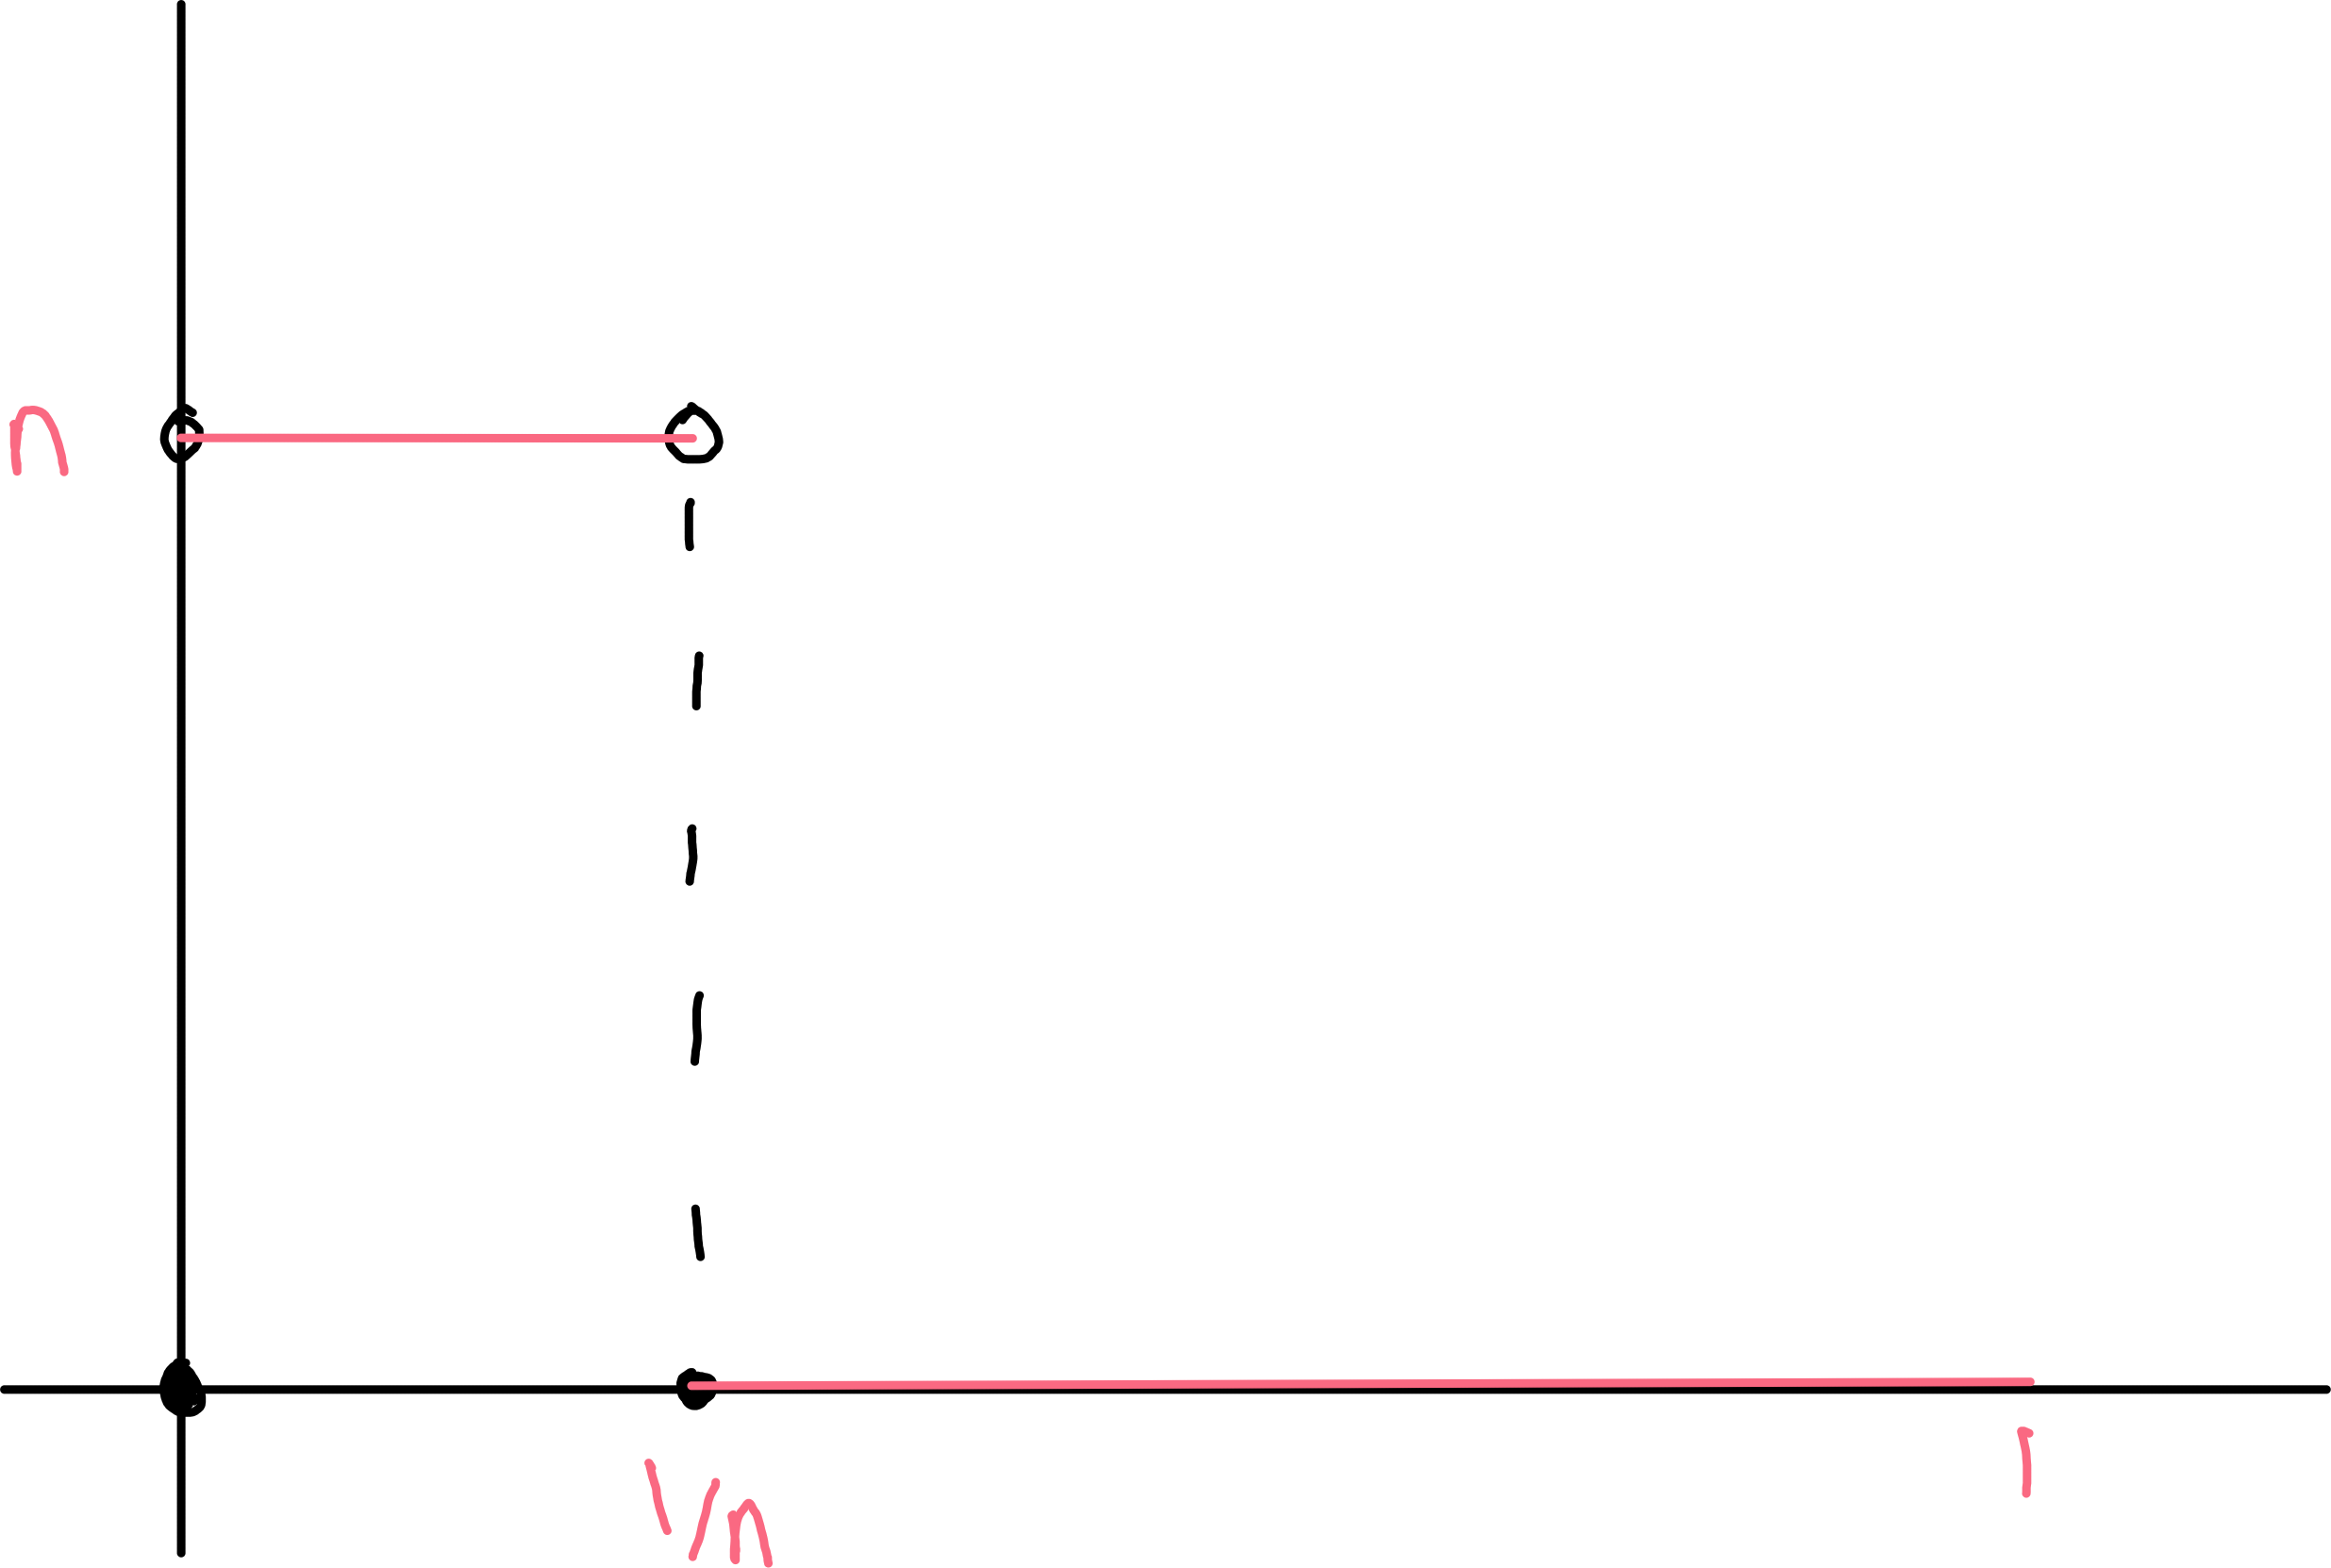
\includegraphics[height=5cm]{01-pointwise2} 
    \par}
    \begin{align*}
        f_n(x) &= \begin{cases}
            n & 0 < x < \frac{1}{n} \\
            0 & \text{otherwise}
        \end{cases}.
    \end{align*} 
    \end{example} 

    Better definition:
    \begin{definition}[Uniform convergence]
        Let $X \subset \mathbb{R}$, $f_n : X \to \mathbb{R}$ ($n \geq 1$), $f: X \to \mathbb{R}$.
        We say $(f_n)$ \vocab{converges uniformly} to $f$ and write $f_n \to f$ uniformly if $\forall \; \epsilon > 0 \ \exists \; N \ \forall \; x \in X \ \forall \; n \geq N \ |f_n(x) - f(x)| < \epsilon$.
    \end{definition} 

    cf $f_n \to f$ pointwise: $\forall \; \epsilon > 0 \ \forall \; x \in X \ \exists \; N \ \forall \; n \geq N \ |f_n(x) - f(x)| < \epsilon$. (We have swapped the $\forall \; x \in x$ and $\exists \; N$).
    Pointwise convergence allows for $N$ to be a function of $x$ whilst uniform convergence requires $N$ to work for all $x$ even the worst case.
    In particular, $f_n \to f$ uniformly $\implies f_n \to f$ pointwise.

    \begin{center}
        \tikzset{every picture/.style={line width=0.75pt}} %set default line width to 0.75pt        
    
        \begin{tikzpicture}[x=0.75pt,y=0.75pt,yscale=-1,xscale=1]
        %uncomment if require: \path (0,300); %set diagram left start at 0, and has height of 300
        
        %Straight Lines [id:da15070589522945865] 
        \draw    (120,42) -- (120,228) ;
        \draw [shift={(120,230)}, rotate = 270] [color={rgb, 255:red, 0; green, 0; blue, 0 }  ][line width=0.75]    (10.93,-3.29) .. controls (6.95,-1.4) and (3.31,-0.3) .. (0,0) .. controls (3.31,0.3) and (6.95,1.4) .. (10.93,3.29)   ;
        \draw [shift={(120,40)}, rotate = 90] [color={rgb, 255:red, 0; green, 0; blue, 0 }  ][line width=0.75]    (10.93,-3.29) .. controls (6.95,-1.4) and (3.31,-0.3) .. (0,0) .. controls (3.31,0.3) and (6.95,1.4) .. (10.93,3.29)   ;
        %Straight Lines [id:da06812433005878815] 
        \draw    (338,200) -- (92,200) ;
        \draw [shift={(90,200)}, rotate = 360] [color={rgb, 255:red, 0; green, 0; blue, 0 }  ][line width=0.75]    (10.93,-3.29) .. controls (6.95,-1.4) and (3.31,-0.3) .. (0,0) .. controls (3.31,0.3) and (6.95,1.4) .. (10.93,3.29)   ;
        \draw [shift={(340,200)}, rotate = 180] [color={rgb, 255:red, 0; green, 0; blue, 0 }  ][line width=0.75]    (10.93,-3.29) .. controls (6.95,-1.4) and (3.31,-0.3) .. (0,0) .. controls (3.31,0.3) and (6.95,1.4) .. (10.93,3.29)   ;
        %Curve Lines [id:da9975807479144934] 
        \draw [color={rgb, 255:red, 74; green, 144; blue, 226 }  ,draw opacity=1 ]   (140,140) .. controls (180,110) and (190,140) .. (230,110) .. controls (270,80) and (295,145) .. (320,120) ;
        %Curve Lines [id:da8386196196350342] 
        \draw [color={rgb, 255:red, 208; green, 2; blue, 27 }  ,draw opacity=1 ] [dash pattern={on 4.5pt off 4.5pt}]  (140,127) .. controls (180,97) and (190,127) .. (230,97) .. controls (270,67) and (295,132) .. (320,107) ;
        %Curve Lines [id:da7136000427009845] 
        \draw [color={rgb, 255:red, 208; green, 2; blue, 27 }  ,draw opacity=1 ] [dash pattern={on 4.5pt off 4.5pt}]  (140,153) .. controls (180,123) and (190,153) .. (230,123) .. controls (270,93) and (295,158) .. (320,133) ;
        %Shape: Brace [id:dp021850826872210183] 
        \draw  [color={rgb, 255:red, 208; green, 2; blue, 27 }  ,draw opacity=1 ] (172,125.25) .. controls (173.71,125.25) and (174.57,124.39) .. (174.57,122.68) -- (174.57,122.68) .. controls (174.57,120.23) and (175.43,119) .. (177.15,119) .. controls (175.43,119) and (174.57,117.77) .. (174.57,115.32)(174.57,116.43) -- (174.57,115.32) .. controls (174.57,113.61) and (173.71,112.75) .. (172,112.75) ;
        %Curve Lines [id:da39763918210258864] 
        \draw    (140,150) .. controls (180,120) and (200,130) .. (240,100) .. controls (280,70) and (271,135.75) .. (290,121) .. controls (309,106.25) and (295,155) .. (320,130) ;
        
        % Text Node
        \draw (177,119) node [anchor=west] [inner sep=0.75pt]  [color={rgb, 255:red, 208; green, 2; blue, 27 }  ,opacity=1 ]  {$\varepsilon $};
        % Text Node
        \draw (322,116.6) node [anchor=south west] [inner sep=0.75pt]  [color={rgb, 255:red, 74; green, 144; blue, 226 }  ,opacity=1 ]  {$f$};
        % Text Node
        \draw (321,130.4) node [anchor=north west][inner sep=0.75pt]  [color={rgb, 255:red, 0; green, 0; blue, 0 }  ,opacity=1 ]  {$f_{n}$};
        
        
        \end{tikzpicture}
        
    
    \end{center}

    Equivalently, $f_n \to f$ uniformly if for sufficiently large $n$ $f_n - f$ is bounded and $\sup_{x \in X} |f_n - f| \to 0$.

    \begin{theorem}[A uniform limit of cts functions is cts]
        Let $X \subset \mathbb{R}$, let $f_n: X \to \mathbb{R}$ be continuous ($n \geq 1$) and let $f_n \to f: X \to \mathbb{R}$ uniformly.
        Then $f$ is cts.
    \end{theorem} 

    \begin{proof}
        Let $x \in X$.
        Let $\epsilon > 0$.
        As $f_n \to f$ uniformly, we can find $N$ s.t. $\forall \; n \geq N \ \forall \; y \in X \ |f_n(y) - f(y)| < \epsilon$.
        In particular, $\forall \; y \in X \ |f_N(y) - f(y)| < \epsilon$.
        As $f_N$ is cts, we can find $\delta > 0$ s.t. $\forall \; y \in X,\ |y - x| < \delta \implies |f_N(y) - f_N(x)| < \epsilon$.
        Now let $y \in X$ with $|y - x| < \delta$.
        Then
        \begin{align*}
            |f(y) - f(x)| &\leq |f(y) - f_N(y)| + |f_N(y) - f_N(x)| + |f_N(x) - f(x)|\footnote{The core of this proof is this inequality.} \\
            &< \epsilon + \epsilon + \epsilon = 3\epsilon.
        \end{align*} 
        Hence $f$ is cts.
    \end{proof} 

    \begin{remark}
        This is often called a `$3\epsilon$ proof' (or an $\frac{\epsilon}{3}$ proof).
    \end{remark} 

    \begin{theorem}
        Let $f_n: [a, b] \to \mathbb{R}$ ($n \geq 1$) be integrable and let $f_n \to f: [a, b] \to \mathbb{R}$ uniformly.
        Then $f$ is integrable and $\int_a^b f_n \to \int_a^b f$ as $n \to \infty$.
    \end{theorem} 

    \begin{proof}
        As $f_n \to f$ uniformly, we can pick $n$ suff. large s.t. $f_n - f$ is bounded.
        Also $f_n$ is bounded (as integrable).
        So by triangle inequality, $f = (f - f_n) + f_n$ is bounded.
        Let $\epsilon > 0$.
        As $f_n \to f$ uniformly there is some $N$ s.t. $\forall \; n \geq N \ \forall \; x \in [a, b]$ we have $|f_n(x) - f(x)| < \epsilon$. \\
        In particular, $\forall \; x \in [a, b] \ |f_N(x) - f(x)| < \epsilon$.

        By Riemann's criterion, there is some dissection $\mathcal{D}$ of $[a, b]$ for which $S(f_n, \mathcal{D}) - s(f_n, \mathcal{D}) < \epsilon$.
        Let $\mathcal{D} = \{x_0, x_1, x_2, \dots, x_k\}$ where $a = x_0 < x_1 < \dots < x_k = b$.
        Now \begin{align*}
            S(f, \mathcal{D}) &= \sum_{i=1}^{k}  (x_i - x_{i-1}) \sup_{x \in [x_{i-1}, x_i]} f(x) \\
            &\leq \sum_{i=1}^{k}  (x_i - x_{i-1}) \sup_{x \in [x_{i-1}, x_i]} (f_N(x) + \epsilon) \\
            &= \sum_{i=1}^{k}  (x_i - x_{i-1}) \left( \left( \sup_{x \in [x_{i-1}, x_i]} f_N(x) \right) + \epsilon\right) \\
            &= \sum_{i=1}^{k}  (x_i - x_{i-1}) \sup_{x \in [x_{i-1}, x_i]} f_N(x) + \sum_{i=1}^{k} (x_i - x_{i-1}) \epsilon \\
            &= S(f_N, \mathcal{D}) + (b - a)\epsilon.
        \end{align*} 
        That is $S(f, \mathcal{D}) \leq S(f_N, \mathcal{D}) + (b - a)\epsilon$.
        Similarly $s(f, \mathcal{D}) \geq s(f_N, \mathcal{D}) - (b - a)\epsilon$.
        Hence
        \begin{align*}
            S(f, \mathcal{D}) - s(f, \mathcal{D}) &\leq S(f_N, \mathcal{D}) - s(f_N, \mathcal{D}) + 2(b - a) \epsilon \\
            &< (2(b-a) + 1) \epsilon
        \end{align*} 
        But $2(b-a) + 1$ is a constant so $(2(b-a) + 1) \epsilon$ can be made arbitrarily small.
        Hence by Riemann's criterion, $f$ is integrable over $[a, b]$.

        Now, for any $n$ suff. large that $f_n - f$ is bounded, 
        \begin{align*}
            \left| \int_a^b f_n - \int_a^b f \right| &= \left| \int_a^b (f_n - f) \right| \\
            &\leq \int_a^b |f_n - f| \\
            &\leq (b - a) \sup_{x \in [a, b]} |f_n - f| \\
            &\to 0 \text{ as } n \to \infty \text{ since $f_n \to f$ uniformly.}\footnote{Note we said that $f_n \to f$ uniformly if $\sup |f_n - f| \to 0$.}
        \end{align*} 
    \end{proof} 

    \section{Metric Spaces}
    \section{Topological Spaces}
    \part{Generalizing differentiation}
\end{document}